\documentclass{beamer}

\usepackage[utf8]{inputenc}
\usepackage{default}
\usepackage[french]{babel}
\usepackage[utf8]{inputenc}
\usepackage{multicol}
\usepackage{color}
\usepackage[absolute,overlay]{textpos}
\usepackage{tikz}
\usetikzlibrary{arrows,automata}
\usepackage{float}
\usepackage{amsfonts}

\usetheme{Bergen}

\definecolor{example}{RGB}{44, 62, 80}
\definecolor{warning}{RGB}{211, 84, 0}
\definecolor{struct}{RGB}{46, 204, 113}

\setbeamercolor{structure}{fg=struct}
\setbeamercolor{block title alerted}{fg=warning}
\setbeamercolor{block title example}{fg=example}

\def\insertauthorindicator{Qui ?}
\def\insertdateindicator{Quand ?}

\title{Micro architecture de l'ARM v2A}
\author{
  Laniel Francis\\
  \href{mailto:francis.laniel@etu.upmc.fr}{francis.laniel@etu.upmc.fr}
}

\begin{document}
	\maketitle
	\begin{frame}
		\frametitle{L'ARM v2A}
		\framesubtitle{Présentation}
		\begin{block}{Architecture}
			32 bits
		\end{block}
		\begin{block}{Pipeline}
			5 étages :
			\begin{itemize}
				\item IFETCH
				\item DECOD
				\item EXE
				\item MEM
				\item WBK
			\end{itemize}
		\end{block}
	\end{frame}
	
	\begin{frame}
		\frametitle{L'ARM v2A}
		\framesubtitle{Jeu d'instruction}
		\begin{block}{Flags}
			\begin{itemize}
				\item N
				\item Z
				\item C
				\item V
			\end{itemize}
		\end{block}

		\begin{exampleblock}{Mise à jour}
			\begin{semiverbatim}
				SUB\alert{S} R8, R9, R10
				
				CMP R11, R12
			\end{semiverbatim}
		\end{exampleblock}

		
		\begin{exampleblock}{Conditions}
			\begin{semiverbatim}
				ADD\alert{EQ} R4, R5, R6
			\end{semiverbatim}
		\end{exampleblock}
	\end{frame}
	
	\begin{frame}
		\frametitle{IFETCH}
		\begin{figure}[H]
			\centering
			\def\svgwidth{\columnwidth}
			\tiny{
				\input{IFETCH.pdf_tex}
			}
			\caption{Schéma de l'étage IFETCH (les couleurs servent uniquement à clarifier le dessin)}
		\end{figure}
	\end{frame}
	
	\begin{frame}
		\frametitle{IFETCH}
		\framesubtitle{Finalité}
		\begin{itemize}
			\item Gestion du PC
			\item En étroite relation avec le cache instruction
		\end{itemize}

	\end{frame}

	\begin{frame}
		\frametitle{DECOD}
		\framesubtitle{Instructions}
		\begin{figure}
			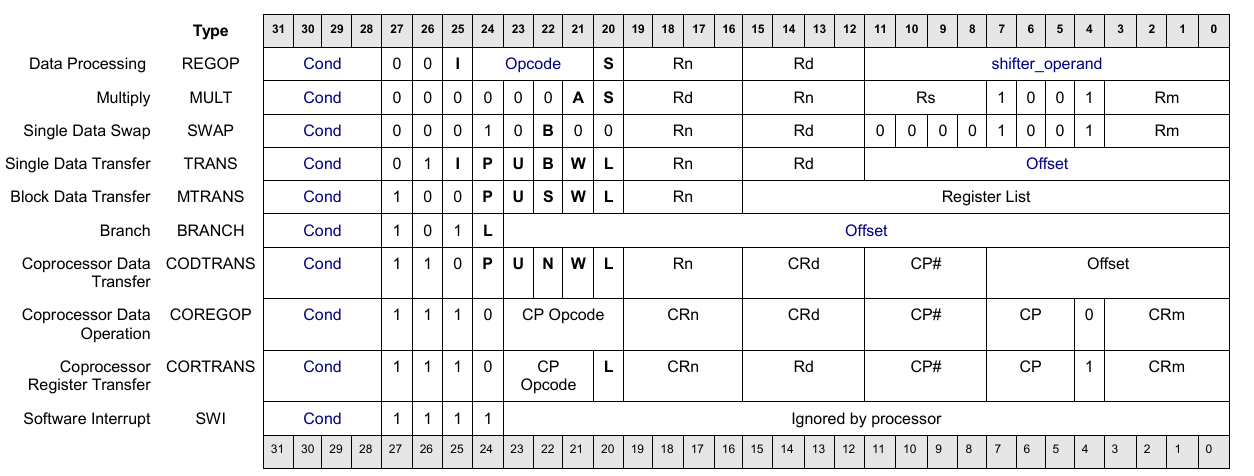
\includegraphics[width=\textwidth]{instructions}
			\caption{Les différents types d'instruction}
		\end{figure}
		\begin{itemize}
			\item $I_{25}$ \checkmark
			\item $L_{24}$ \checkmark
			\item $U_{23}$
			\item $B_{22}$ \checkmark
			\item $A_{21}$ \checkmark
			\item $L_{20}$ \checkmark
			\item $S_{20}$ \checkmark
		\end{itemize}
	\end{frame}
	
	\begin{frame}
		\frametitle{DECOD}
		\framesubtitle{Instructions}
		\begin{figure}[H]
			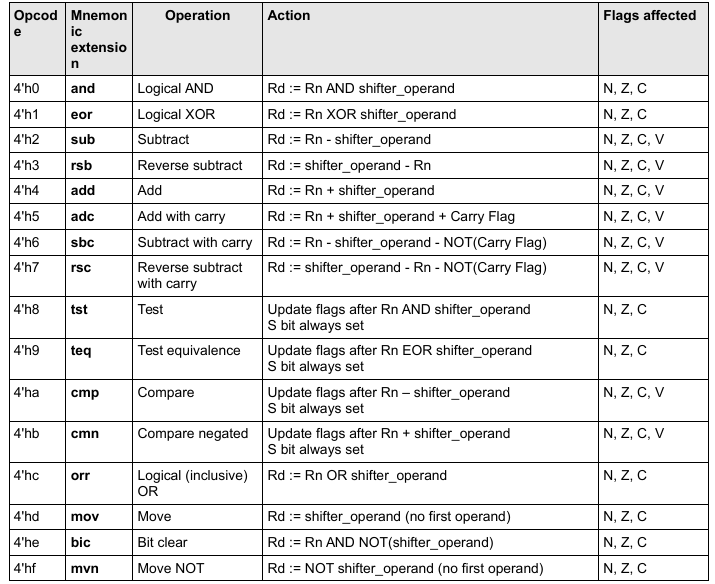
\includegraphics[width=\textwidth]{regop}
			\caption{Les différentes \textbf{REGOP}}
		\end{figure}
	\end{frame}
	
	\begin{frame}
		\frametitle{DECOD}
		\framesubtitle{Machine à état}
		\begin{figure}[H]
			\tiny{
				\begin{tikzpicture}[->, >= stealth, shorten >= 1pt, auto, node distance = 2cm, semithick, initial text = $\overline{RESET\_N}$, initial where = right]
					\tikzstyle{every state} = [fill = white, draw = black, text = black]

					\node [state] (A) {RUN};
					\node [state] (B) [right of = A] {ADR};
					\node [state] (C) [below of = A] {OPWAIT};
					\node [state] (D) [left of = A] {MTRANS};
					\node [state] (E) [above left of = A] {MUL};
					\node [state] (F) [above of = A] {SWAP};
					\node [state] (G) [below of = B] {ADR PC};
					\node [state] (H) [right of = B] {LPC};
					\node [initial, state] (I) [above of = B] {FETCH}; 
					
					\pause

					\path (A) edge [yellow, in = -30, out = -60, loop] node [yellow, pos = 0.33, sloped] {OPOK} (A)
						edge node {BRANCH} (B)
						edge node [sloped, pos = 0.1] {$\overline{OPOK}$} (C)
						edge node {} (D)
						edge [bend left, red] node [red, pos=0.8] {MUL} (E)
						edge node [sloped, pos=0.8] {SWAP} (F)
						edge [bend left] node {} (G)
						(B) edge node {} (I)
						(C) edge [loop left] node {$\overline{OPOK}$} (C)
						edge [blue, bend left] node [blue] {OPOK} (A)
						edge [green] node [green, sloped, pos = 0.9] {OPOK.BRANCH} (B)
						edge node {} (D)
						edge node {} (E)
						(D) edge [loop left] node {} (D)
						edge node {} (A)
						edge node {} (C)
						(E) edge [loop left] node {$\overline{MULOK}$} (E)
						edge node [sloped, pos=0.1] {MULOK} (A)
						(F) edge [loop left] node {$\overline{SWAPOK}$} (F)
						edge [bend left] node [pos = 0.1] {SWAPOK} (A)
						(G) edge node {} (H)
						(H) edge node {} (I)
						(I) edge node {} (A);
				\end{tikzpicture}
				\caption{Machine à état de DECOD (les couleurs servent uniquement à clarifier le dessin)}
			}
		\end{figure}
		\begin{alertblock}{Attention}
			Code écrit mais non vérifié, par conséquent ça ne fonctionne pas
		\end{alertblock}
	\end{frame}
	
	\begin{frame}
		\frametitle{EXE}
		\framesubtitle{Schéma}
		\begin{figure}[H]
			\centering
			\def\svgwidth{0.9\columnwidth}
			\tiny{
				\input{EXE.pdf_tex}
			}
			\caption{Schéma de l'étage EXE}
		\end{figure}
	\end{frame}
	
	\begin{frame}
		\frametitle{EXE}
		\framesubtitle{Vraies opérations}
		\begin{itemize}
			\item AND
			\item OR
			\item XOR
			\item ADD
		\end{itemize}
	\end{frame}

	\begin{frame}
		\frametitle{EXE}
		\framesubtitle{Décalages}
		\begin{itemize}
			\item LSL \checkmark
			\item LSR \checkmark
			\item ASR
			\item ROR \checkmark
			\item RRX \checkmark
		\end{itemize}
		\begin{alertblock}{ASR}
			sign\_op2 calculé trop ``tôt''
		\end{alertblock}
	\end{frame}
	
	\begin{frame}
		\frametitle{EXE}
		\framesubtitle{Addition}
		\begin{figure}[H]
			\centering
			\def\svgwidth{\columnwidth}
			\scriptsize{
				\input{Full-adder.pdf_tex}
			}
			\caption{Schéma d'un additionneur complet}
		\end{figure}
	\end{frame}

	
	\begin{frame}
		\frametitle{MEM}
		\begin{itemize}
			\item Relié au cache de données
			\item Opérations selon $B_{22}$ et $L_{20}$
			\item Adresse calculée dans EXE
		\end{itemize}
		\begin{alertblock}{Attention}
			Non testé
		\end{alertblock}
	\end{frame}
	
	\begin{frame}
		\frametitle{Conclusion}
		\framesubtitle{Échec}
		\begin{itemize}
			\item Décodage des instructions
			\item Calcul de l'étage EXE
		\end{itemize}
		\begin{alertblock}{Attention}
			Étages non reliés, aucune interaction entre eux
		\end{alertblock}
	\end{frame}

	\begin{frame}
		\frametitle{Conclusion}
		\framesubtitle{Mais...}
		\begin{itemize}
			\item Initiation au VHDL
			\item GHDL
			\item GTKWAVE
			\item \LaTeX
			\item Alliance
		\end{itemize}
	\end{frame}
\end{document}